\begin{frame}{Validação no LTspice: diagramas de Bode}
  \begin{columns}[T,onlytextwidth]
    \begin{column}{0.31\textwidth}
      \centering
      \textbf{Sem carga}

      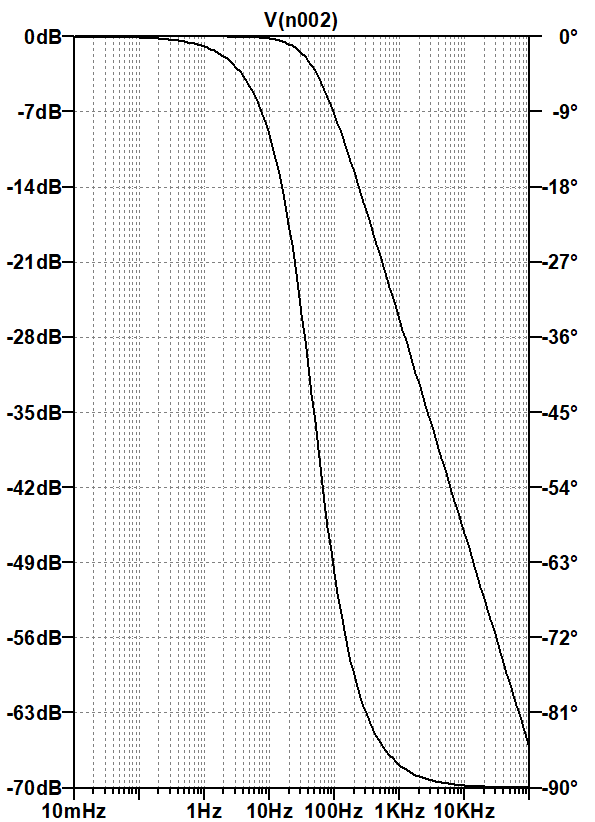
\includegraphics[height=0.52\textheight,width=\linewidth,keepaspectratio]{slides/img/ltspice_bode_1.png}

      \small Patamar próximo de $0\,\mathrm{dB}$.
    \end{column}
    \begin{column}{0.31\textwidth}
      \centering
      \textbf{Carga direta}

      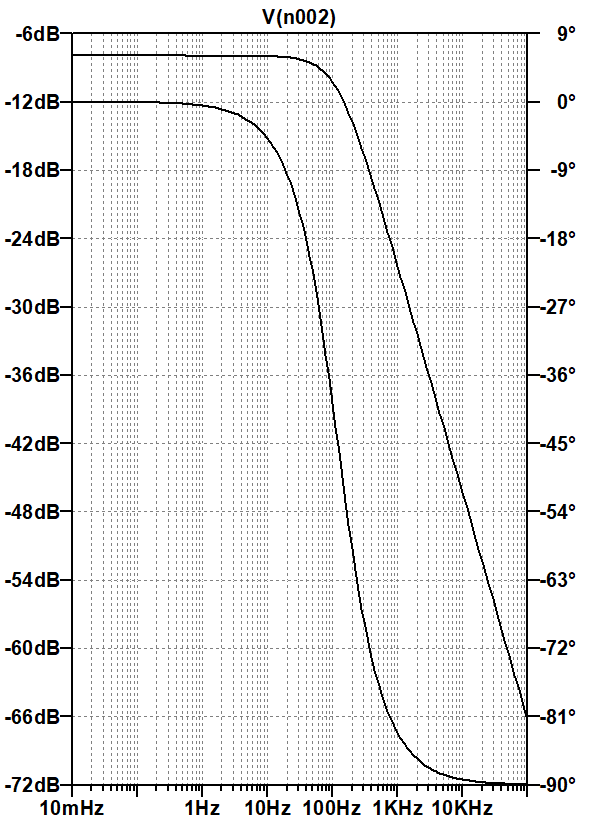
\includegraphics[height=0.52\textheight,width=\linewidth,keepaspectratio]{slides/img/ltspice_bode_2.png}

      \small Patamar atenuado e corte deslocado.
    \end{column}
    \begin{column}{0.31\textwidth}
      \centering
      \textbf{Com buffer}

      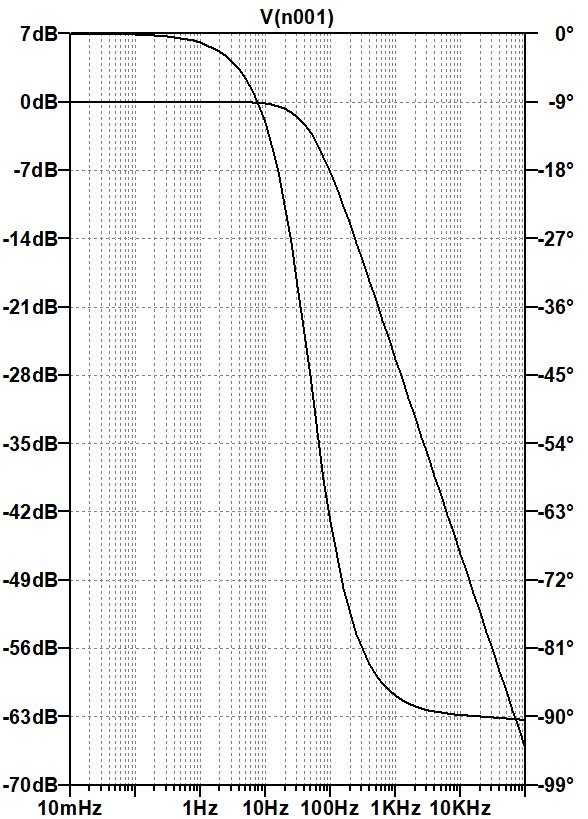
\includegraphics[height=0.52\textheight,width=\linewidth,keepaspectratio]{slides/img/ltspice_bode_3.png}

      \small Recuperação da resposta sem carga.
    \end{column}
  \end{columns}

  \vspace{0.10cm}
  \centering\scriptsize
  Capturas originais das simulações do projeto nominal.
  A comparação é qualitativa; magnitude e fase aparecem no mesmo painel.
\end{frame}
